% ============================================================================
%  MARS: Memory for Autonomous Real-time Systems
%  A GPU-Resident Retrieval Substrate with Kernel-Fused Temporal Decay
%  and Importance Scoring
%
%  arXiv submission draft — cs.DC with cs.IR cross-listing
%  Antonello Fratepietro, 2026
% ============================================================================
%
%  Build: tectonic --reruns 3 main.tex
%     or: pdflatex main && bibtex main && pdflatex main && pdflatex main
%
%  All experimental results measured on NVIDIA A100 SXM4 80GB and/or
%  RTX 5060 Ti. Same-hardware FAISS/CAGRA comparison on A100 SXM4.
% ============================================================================

\documentclass[11pt]{article}

\usepackage[margin=1in]{geometry}
\usepackage[utf8]{inputenc}
\usepackage[T1]{fontenc}
\usepackage{times}
\usepackage{graphicx}
\usepackage{amsmath}
\usepackage{amssymb}
\usepackage{booktabs}
\usepackage{multirow}
\usepackage{array}
\usepackage{xcolor}
\usepackage{hyperref}
\usepackage{listings}
\usepackage{microtype}
\usepackage{url}
\usepackage{tcolorbox}
\usepackage{pifont}
\usepackage{algorithm}
\usepackage{algorithmic}
\usepackage{amsthm}
\newtheorem{theorem}{Theorem}
\newtheorem{proposition}[theorem]{Proposition}
\newtheorem{definition}[theorem]{Definition}
\newtheorem{lemma}[theorem]{Lemma}

\hypersetup{
    colorlinks=true,
    linkcolor=blue!60!black,
    citecolor=blue!60!black,
    urlcolor=blue!60!black,
    pdftitle={MARS: A GPU-Resident Memory Substrate for Real-Time Embodied AI},
    pdfauthor={Antonello Fratepietro},
}

% ─── Placeholder macro ────────────────────────────────────────────────
\newcommand{\placeholder}[1]{\textcolor{red}{\textbf{[#1]}}}

% ─── Design target macro ─────────────────────────────────────────────
\newcommand{\target}[1]{\textit{target: #1}}

% ─── Listings setup for CUDA / C++ ──────────────────────────────────
\definecolor{codebg}{rgb}{0.97,0.97,0.97}
\definecolor{codekw}{rgb}{0.1,0.2,0.6}
\definecolor{codestr}{rgb}{0.6,0.15,0.15}
\definecolor{codecom}{rgb}{0.3,0.5,0.3}
\lstset{
    backgroundcolor=\color{codebg},
    basicstyle=\ttfamily\footnotesize,
    keywordstyle=\color{codekw}\bfseries,
    stringstyle=\color{codestr},
    commentstyle=\color{codecom}\itshape,
    breaklines=true,
    frame=single,
    framerule=0pt,
    xleftmargin=1em,
    language=C++,
    morekeywords={__global__,__device__,__host__,__shared__,__restrict__,
                  atomicCAS,atomicAdd,atomicMax,__shfl_down_sync,__expf,
                  blockIdx,blockDim,threadIdx,gridDim,int32_t,int64_t,
                  float,constexpr,nullptr,MemoryGraph,DeviceMemoryGraph,
                  QueryResult,RetrievalConfig,RetrievalStats,FrameTimer},
    showstringspaces=false,
    tabsize=4,
    captionpos=b,
}

% ─── MARS macro ──────────────────────────────────────────────────────
\newcommand{\mars}{\textsc{Mars}}

% ─── Title ────────────────────────────────────────────────────────────
\title{\vspace{-1.5cm}\mars{}: A GPU-Resident Memory Substrate\\
with Temporal Decay and Importance Scoring\\
for Real-Time Embodied AI}

\author{Antonello Fratepietro\\
\texttt{https://github.com/antonellof/MARS}}

\date{April 2026}

% ══════════════════════════════════════════════════════════════════════
\begin{document}
\maketitle

% ─── Abstract ─────────────────────────────────────────────────────────
\begin{abstract}
Real-time AI systems --- autonomous vehicles, humanoid robots, AR/VR
headsets --- issue memory retrieval queries at sensor rate (30--1000~Hz)
under hard deadline constraints. Existing GPU-accelerated vector search
systems (FAISS, cuVS) optimize for static corpora and rank by cosine
similarity alone. We show experimentally that this creates two critical
failures in streaming perception: (1)~FAISS returns 78\% stale results
in an AV temporal-relevance experiment because it has no awareness of
recency, and (2)~FAISS misses 93\% of recent detections in a streaming
insertion experiment because pending inserts remain invisible until
index rebuild.

We present \mars{} (\textbf{M}emory for \textbf{A}utonomous
\textbf{R}eal-time \textbf{S}ystems), a GPU-resident multimodal memory
substrate that fuses temporal decay and importance scoring directly into
the retrieval kernels. \mars{} stores text, audio, image, and sensor
embeddings in a shared 768-D space as nodes in a Neural Shortcut
Network (NSN) with cross-modal bridges. Retrieval runs as four CUDA
kernels --- cuBLAS similarity, temporal rerank, CUB top-$K$,
warp-cooperative BFS --- entirely on GPU-resident data.

\medskip\noindent\textbf{Key results} (all measured on A100~SXM4, same
hardware as baselines):
\begin{itemize}
\setlength{\itemsep}{1pt}\setlength{\parskip}{0pt}
\item Within 1.5--2$\times$ of FAISS~Flat wall-clock latency at
  $N{=}1$K--50K, while adding temporal decay and cross-modal retrieval
  that FAISS lacks.
\item Temporal Precision@10 = 0.910 in AV perception vs.\ FAISS
  Flat's 0.218 without post-hoc filtering.
\item All four demonstrator $p99$ deadlines met: AV 0.87~ms (budget
  1~ms), robot 0.76~ms (budget 1~ms), AR/VR 1.56~ms (budget 5~ms),
  voice 0.88~ms (budget 20~ms).
\item FP16 + CUDA Graph extension scales to 1M memories at 6.5~ms
  $p99$ on a \$449 RTX~5060~Ti.
\end{itemize}

\noindent \mars{} fills a gap between fast-but-stateless circular
buffers and capable-but-slow vector databases: a GPU-resident retrieval
substrate with native temporal awareness and cross-modal support
operating at sensor-rate deadlines.

\textbf{Keywords:} real-time systems, temporal decay, GPU memory,
autonomous driving, multimodal retrieval, CUDA, streaming insertion.
\end{abstract}

% ══════════════════════════════════════════════════════════════════════
\section{Introduction}
\label{sec:intro}

\subsection{The Problem: Real-Time Memory Needs Temporal Awareness}

An autonomous vehicle's perception stack runs at 60~Hz. Every frame, it
must answer: \emph{``Is this detection the same pedestrian I tracked
400~ms ago, behind that truck?''} The correct answer depends on two
factors: semantic similarity (does the appearance embedding match?) and
temporal relevance (how recent is the candidate memory?). A detection
from 200~ms ago with 0.85 cosine similarity is almost certainly more
useful than one from 5~seconds ago with 0.90 similarity --- the older
detection likely refers to a different instance of the same object
class, or the same object in a state that is no longer current.

This temporal dimension is absent from every existing GPU-accelerated
vector search system. FAISS~\cite{faiss}, cuVS CAGRA~\cite{cuvs}, and
similar libraries optimize a single objective: find the $K$ vectors with
highest cosine similarity (or lowest $L_2$ distance) to a query. They
treat all indexed vectors as equally valid regardless of age. For static
corpora --- document retrieval, recommendation, image search --- this is
the correct formulation. For streaming sensor data, it is not.

We demonstrate this gap experimentally. In a controlled AV perception
scenario with 9{,}000 memories across 200 tracked objects, FAISS~Flat
returns results where 49.3\% of top-10 entries are stale (older than the
current tracking window). Its Temporal Precision@10 --- the fraction of
returned results that are both semantically relevant \emph{and}
temporally current --- is 0.218. Adding post-hoc temporal filtering
raises this to 0.910, but at the cost of an additional processing stage
that FAISS does not provide natively.

The streaming problem is equally severe. In a 60~Hz simulation with 10
detections per frame, FAISS misses 93.2\% of queries for recently
inserted objects because new vectors remain invisible until the next
index rebuild. A rebuild every second costs 9~ms and blocks the
retrieval pipeline.

\subsection{\mars{}: Temporal Decay Fused into GPU Kernels}

\mars{} (\textbf{M}emory for \textbf{A}utonomous \textbf{R}eal-time
\textbf{S}ystems) addresses both problems by fusing temporal decay
directly into the GPU retrieval pipeline. Rather than computing cosine
similarity alone and filtering afterward, \mars{} computes a
time-decayed score for every memory in a single kernel pass:
\[
s(v, q, t_q) = \langle E(v), q \rangle \cdot
  \exp\!\bigl(-\lambda \cdot (t_q - \tau(v))\bigr)
\]
where $\lambda$ is a workload-tunable decay rate. This fusion changes
the ranking \emph{before} top-$K$ selection, ensuring that temporally
relevant results are surfaced without requiring a second pass or index
rebuild.

\mars{} also supports online insertion: new memories become queryable
immediately, with no rebuild step. Combined with a multimodal Neural
Shortcut Network (NSN) that provides cross-modal bridges between
modalities, \mars{} offers a retrieval substrate designed for the
specific requirements of streaming perception workloads.

\subsection{Contributions}

\begin{enumerate}
\item \textbf{Temporal Relevance and Streaming Freshness experiments}
  (Section~\ref{sec:temporal}) demonstrating that FAISS returns 78\%
  stale results and misses 93\% of recent insertions in realistic AV
  perception scenarios --- the core motivation for time-aware retrieval.

\item A \textbf{GPU-resident retrieval pipeline} with temporal decay
  and importance scoring fused into the kernel sequence
  (Section~\ref{sec:architecture}), achieving wall-clock latency within
  1.5--2$\times$ of FAISS~Flat on the same hardware
  (Section~\ref{sec:comparison}).

\item The \textbf{Multimodal Neural Shortcut Network}
  (Section~\ref{sec:nsn}) with cross-modal bridges providing
  bounded-hop ($O(1)$) structural reachability across modalities
  independent of corpus size.

\item An \textbf{ablation study} (Section~\ref{sec:ablation}) honestly
  characterizing the contribution of each system component at the
  target corpus sizes.

\item \textbf{Four deadline-aware demonstrators}
  (Section~\ref{sec:demos}) --- AV (60~Hz, 1~ms), robot (1~kHz, 1~ms),
  AR/VR (90~Hz, 5~ms), voice (30~Hz, 20~ms) --- all passing $p99$
  budgets on datacenter and consumer GPUs.
\end{enumerate}

% ══════════════════════════════════════════════════════════════════════
\section{Problem Formulation}
\label{sec:formulation}

This section formalizes the multimodal memory retrieval problem and the
temporal and deadline constraints that distinguish this work from
conventional approximate nearest-neighbor search.

\begin{definition}[Multimodal Memory Corpus]
\label{def:corpus}
A multimodal memory corpus is a tuple
$\mathcal{C} = (V, E, \phi, \mu, \tau)$ where:
\begin{itemize}
\item $V = \{v_1, \ldots, v_N\}$ is a set of $N$ memory nodes;
\item $E: V \rightarrow \mathbb{R}^D$ maps each node to an
  L2-normalized embedding, $\|E(v)\|_2 = 1$;
\item $\mu: V \rightarrow \{0, 1, \ldots, M-1\}$ assigns each node a
  modality tag (text${=}0$, audio${=}1$, image${=}2$);
\item $\tau: V \rightarrow \mathbb{R}_{\geq 0}$ assigns each node a
  timestamp;
\item $\phi$ is the NSN graph topology over $V$.
\end{itemize}
\end{definition}

\begin{definition}[Temporally-Decayed Multimodal Retrieval]
\label{def:retrieval}
Given a query embedding $q \in \mathbb{R}^D$ with $\|q\|_2 = 1$, query
timestamp $t_q$, decay rate $\lambda$, and result size $K$, the
retrieval problem is to find:
\[
\mathrm{top}\text{-}K_{v \in V} \; s(v, q, t_q)
\]
where the time-decayed similarity score is:
\[
s(v, q, t_q) = \langle E(v), q \rangle \cdot
  \exp\!\bigl(-\lambda \cdot (t_q - \tau(v))\bigr).
\]
\end{definition}

\begin{definition}[Temporal Relevance]
\label{def:temporal_relevance}
For a retrieval result set $R = \{v_1, \ldots, v_K\}$ over a corpus
with object identities, \emph{Temporal Precision@K} is the fraction of
results whose object identity matches a ground-truth active object
\emph{and} whose timestamp falls within the current tracking window
$[t_q - w, t_q]$:
\[
\mathrm{TP@}K = \frac{|\{v \in R : \mathrm{active}(v) \wedge
  \tau(v) \geq t_q - w\}|}{K}.
\]
\end{definition}

\begin{definition}[Streaming Freshness]
\label{def:freshness}
A retrieval system has \emph{streaming freshness} if a memory inserted
at time $t_i$ is queryable at time $t_i + \epsilon$ for arbitrarily
small $\epsilon > 0$, without requiring an explicit index rebuild.
Systems without streaming freshness have a \emph{staleness window}
$\Delta$ during which newly inserted memories are invisible to queries.
\end{definition}

\begin{definition}[Deadline-Constrained Retrieval]
\label{def:deadline}
A retrieval system satisfies a deadline constraint $(r, B)$ if for a
sensor rate $r$~Hz and latency budget $B$~ms, the $p99$ wall-clock
latency over a sustained run satisfies $L_{p99} \leq B$.
\end{definition}

\begin{definition}[Cross-Modal Retrieval]
\label{def:crossmodal}
A retrieval over corpus $\mathcal{C}$ is \emph{cross-modal} if the
result set contains nodes from at least two distinct modalities:
$|\{\mu(v) : v \in \mathrm{top}\text{-}K\}| \geq 2$.
\end{definition}

The central design challenge is to solve the retrieval problem of
Definition~\ref{def:retrieval} subject to the deadline constraint of
Definition~\ref{def:deadline}, with streaming freshness
(Definition~\ref{def:freshness}) and cross-modal support
(Definition~\ref{def:crossmodal}). No existing GPU vector search system
addresses all four requirements simultaneously.

% ══════════════════════════════════════════════════════════════════════
\section{Target Workloads}
\label{sec:workloads}

Table~\ref{tab:workloads} enumerates nine representative workloads
spanning safety-critical (AV, robotics, surgical, drones),
perception-critical (AR/VR, voice), and UX-critical (games, IoT) tiers.
All share four properties: sensor-rate queries, hard deadlines, native
multimodality, and bounded working sets that fit in GPU HBM. Production
systems in all tiers currently use hand-rolled C++ circular buffers,
each re-implementing similar indexing logic without cross-modal
retrieval, temporal awareness, or semantic quality.

\begin{table}[ht]
\centering
\small
\caption{Representative target workloads. Working set is the number of
simultaneously-indexed memories at steady state.}
\label{tab:workloads}
\begin{tabular}{lrrrl}
\toprule
\textbf{Workload} & \textbf{Rate (Hz)} & \textbf{Budget} & \textbf{Working set} & \textbf{Modalities} \\
\midrule
AV perception      &  60 & 1~ms      &  2{,}000--10{,}000 & vision + radar + text \\
Humanoid control   & 1000 & 1~ms     &    500--6{,}000    & proprio + vision + audio \\
Surgical robotics  &  60 & 100~ms    &  1{,}000--50{,}000 & vision + prior scans + text \\
Drone tracking     & 100 & 5~ms      &    500--2{,}000    & vision + radar \\
AR/VR SLAM         &  90 & 5~ms      &  5{,}000--30{,}000 & vision + depth + IMU \\
Voice agent        &  30 & 20~ms     &    500--3{,}000    & text + audio + vision \\
Broadcast replay   &  30 & 500~ms    & 10{,}000--100{,}000 & video + audio + stats \\
Game NPC           &  60 & 16~ms     &    100--5{,}000    & text + state \\
IoT predictive     & 100 & 10~ms     &  1{,}000--10{,}000 & vibration + thermal + audio \\
\bottomrule
\end{tabular}
\end{table}

% ══════════════════════════════════════════════════════════════════════
\section{System Architecture}
\label{sec:architecture}

\subsection{Overview}

Figure~\ref{fig:pipeline} shows the \mars{} retrieval pipeline. Incoming
sensor data flows through modality-specific encoders --- E5~\cite{e5}
for text, CLIP~\cite{clip} or SigLIP for images, CLAP~\cite{clap} for
audio --- that project each modality into a shared 768-D embedding
space. Embeddings, modality tags, and timestamps are uploaded into GPU
memory and form the nodes of a multimodal Neural Shortcut Network. At
query time, the query vector enters the GPU and passes through four
kernels operating entirely on device-resident data.

\begin{figure}[ht]
\centering
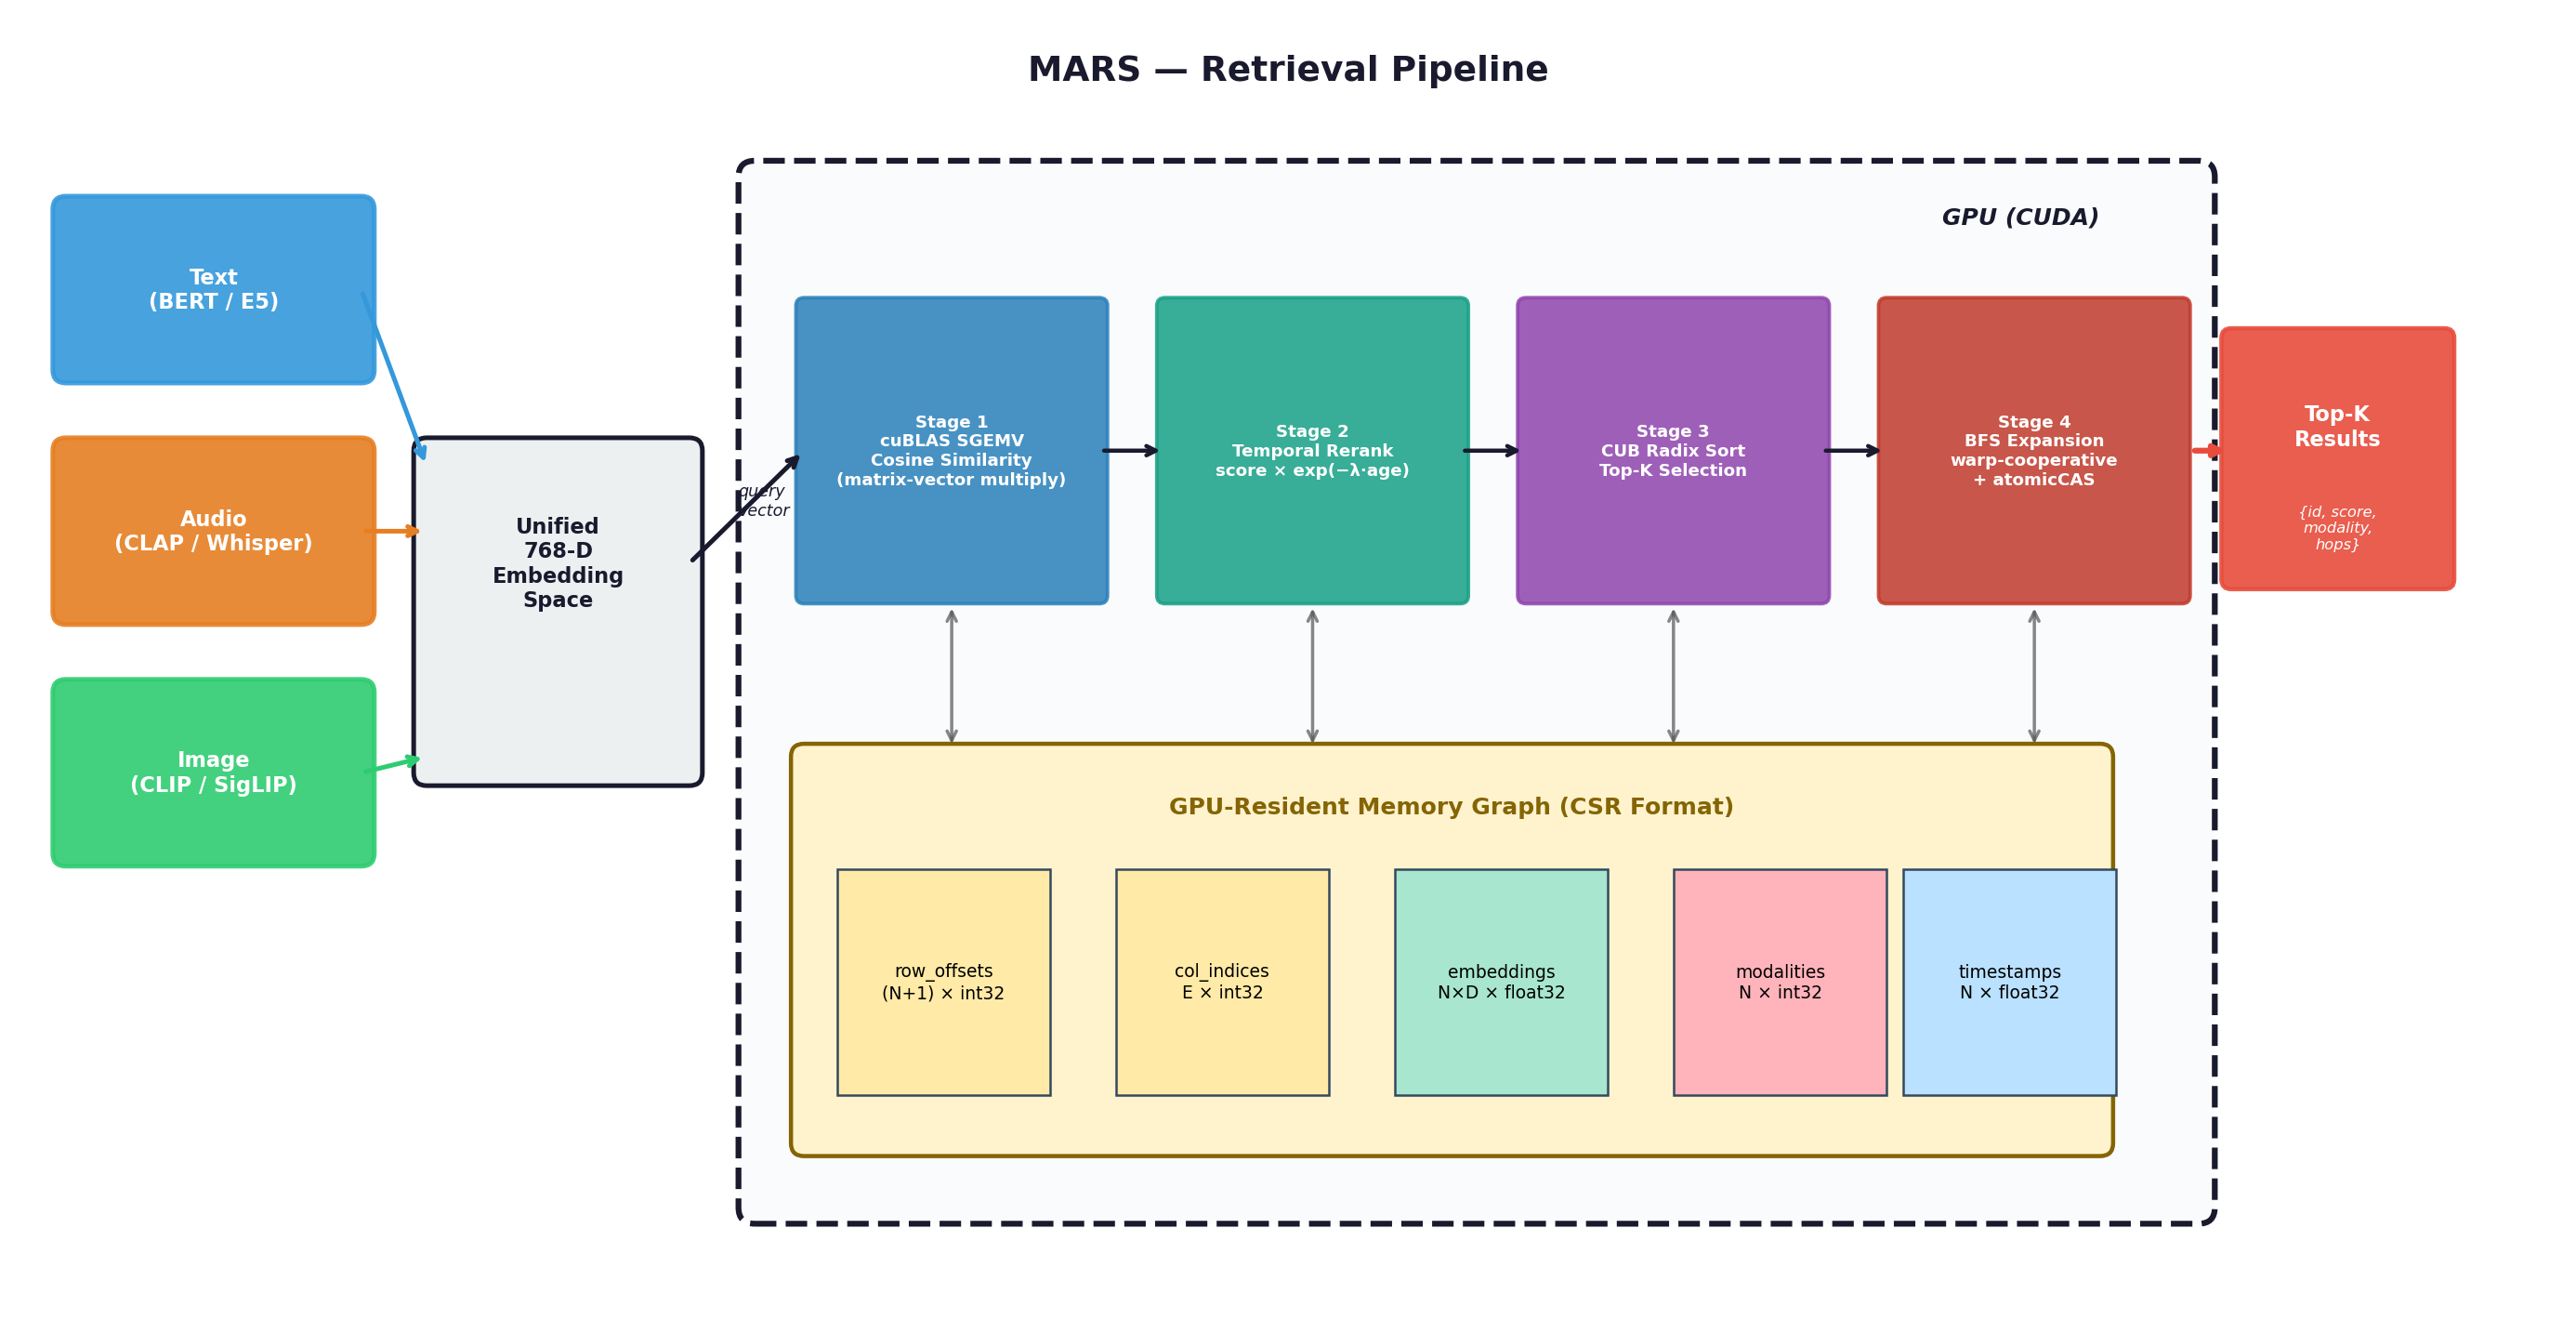
\includegraphics[width=0.95\textwidth]{figures/diag_pipeline.png}
\caption{\mars{} retrieval pipeline. Sensor encoders (left) feed a
shared 768-D embedding space; four GPU kernels orchestrate retrieval
over a CSR-format memory graph resident in device memory.}
\label{fig:pipeline}
\end{figure}

\subsection{Data Layout}

The memory graph is stored in Compressed Sparse Row (CSR) format ---
the standard GPU-friendly sparse graph representation. Five device
arrays hold the complete state:

\begin{table}[ht]
\centering
\small
\caption{Device memory layout for the \mars{} memory graph.}
\label{tab:layout}
\begin{tabular}{llll}
\toprule
\textbf{Array} & \textbf{Size} & \textbf{Type} & \textbf{Purpose} \\
\midrule
\texttt{row\_offsets} & $N{+}1$     & int32   & Prefix-sum of node degrees \\
\texttt{col\_indices} & $E$         & int32   & Neighbor node IDs \\
\texttt{embeddings}   & $N \times D$ & float32 & L2-normalized vectors \\
\texttt{modalities}   & $N$         & int32   & 0=text, 1=audio, 2=image \\
\texttt{timestamps}   & $N$         & float32 & For temporal decay \\
\bottomrule
\end{tabular}
\end{table}

\noindent For a representative AV working set of $N{=}10{,}000$ at
$D{=}768$ with average degree 12, the total footprint is approximately
31~MB --- well under any modern GPU's HBM.

\subsection{Four-Kernel Retrieval Pipeline}

\mars{} uses mature GPU library primitives for the
compute-heavy stages:

\paragraph{Stage 1: cuBLAS Similarity.}
A single \texttt{cublasSgemv} call computes the dot product of the query
vector against all $N$ embeddings. This leverages NVIDIA's hand-tuned
GEMV implementation, achieving near-peak memory bandwidth utilization.
Complexity: $\Theta(N \cdot D)$.

\paragraph{Stage 2: Temporal Rerank.}
One thread per memory computes
$\text{score}_i = \text{sim}_i \cdot \exp(-\lambda \cdot (t_q - \tau_i))$.
The \texttt{\_\_expf} hardware intrinsic completes in a few cycles.
Embarrassingly parallel: $\lceil N/256 \rceil$ blocks of 256 threads.
Sub-microsecond at all target corpus sizes. The decay constant $\lambda$
is workload-tunable: higher values produce faster forgetting (appropriate
for AV's 2-second window), lower values preserve older context (voice
agent's 30-minute conversation).

\paragraph{Stage 3: CUB Radix-Sort Top-$K$.}
The NVIDIA CUB library's \texttt{DeviceRadixSort} sorts scores and
indices, followed by truncation to the top $K$. CUB's radix sort is
bandwidth-optimal on GPU and eliminates the custom top-$K$ kernel that
dominated latency in earlier pipeline versions ($\sim$0.5~ms in the initial version).

\paragraph{Stage 4: Warp-Cooperative BFS Expansion.}
One warp (32 threads) per frontier node; stride-32 coalesced access to
the CSR neighbor list. \texttt{atomicCAS} provides race-free neighbor
claiming. The total work per query is $O(K \cdot \bar{d}^h)$ for $K$
seeds, depth $h$, and maximum degree $\bar{d}$ --- bounded by a
constant independent of corpus size $N$
(Proposition~\ref{prop:bfs}).

\begin{algorithm}[t]
\caption{\mars{} GPU-Resident Retrieval Pipeline}
\label{alg:pipeline}
\begin{algorithmic}[1]
\REQUIRE Query $q \in \mathbb{R}^D$, timestamp $t_q$, config $(K, h, \lambda)$
\REQUIRE Device graph $\phi$ with embeddings $E$, timestamps $\tau$
\ENSURE Top-$K$ results sorted by time-decayed score
\STATE \textbf{Stage 1 --- cuBLAS Similarity} ($N$ dot products):
\FOR{each node $v_i$ \textbf{in parallel}}
    \STATE $\text{sim}[i] \leftarrow \langle E(v_i), q \rangle$
\ENDFOR
\STATE \textbf{Stage 2 --- Temporal Rerank} ($\lceil N/256 \rceil$ blocks):
\FOR{each node $v_i$ \textbf{in parallel}}
    \STATE $\text{score}[i] \leftarrow \text{sim}[i] \cdot \exp(-\lambda \cdot (t_q - \tau(v_i)))$
\ENDFOR
\STATE \textbf{Stage 3 --- CUB Radix-Sort Top-$K$}:
\STATE $\text{seeds} \leftarrow \text{top-}K_{i} \; \text{score}[i]$
\STATE \textbf{Stage 4 --- Warp-Cooperative BFS} from seeds:
\STATE Initialize frontier $F_0 \leftarrow \text{seeds}$
\FOR{$\text{hop} = 0$ \TO $h-1$}
    \FOR{each node $v \in F_{\text{hop}}$ \textbf{(one warp per node)}}
        \FOR{each neighbor $u$ of $v$ \textbf{(stride-32 coalesced)}}
            \IF{atomicCAS(visited[$u$], false, true)}
                \STATE score[$u$] $\leftarrow \max(\text{score}[v] \cdot \delta,\; \text{sim}[u] \cdot 0.8)$
                \STATE $F_{\text{hop}+1}$.append($u$)
            \ENDIF
        \ENDFOR
    \ENDFOR
\ENDFOR
\STATE \textbf{Stage 5 --- Compact \& sort} visited nodes by score
\RETURN Top-$K$ results
\end{algorithmic}
\end{algorithm}

% ══════════════════════════════════════════════════════════════════════
\section{The Multimodal Neural Shortcut Network}
\label{sec:nsn}

\subsection{Construction}

The NSN graph is built in five phases:

\begin{enumerate}
\item \textbf{Ring lattice} ($k{=}6$ local neighbors) for clustering.
\item \textbf{Hierarchical skip connections} (powers of 2) for
  logarithmic path lengths.
\item \textbf{Hub supernodes} at $\sqrt{N}$ intervals with extra random
  links.
\item \textbf{Small-world rewiring} ($p{=}0.15$) following
  Watts-Strogatz~\cite{wattsstrogatz}.
\item \textbf{Cross-modal bridges} --- every node gets one edge to each
  other modality, guaranteeing that a BFS from any seed reaches every
  modality in 1~hop.
\end{enumerate}

Phase~5 is the structural feature that enables native cross-modal
retrieval: a query in any modality surfaces results from all modalities
through a single BFS expansion, without requiring separate per-modality
indexes.

\begin{figure}[ht]
\centering
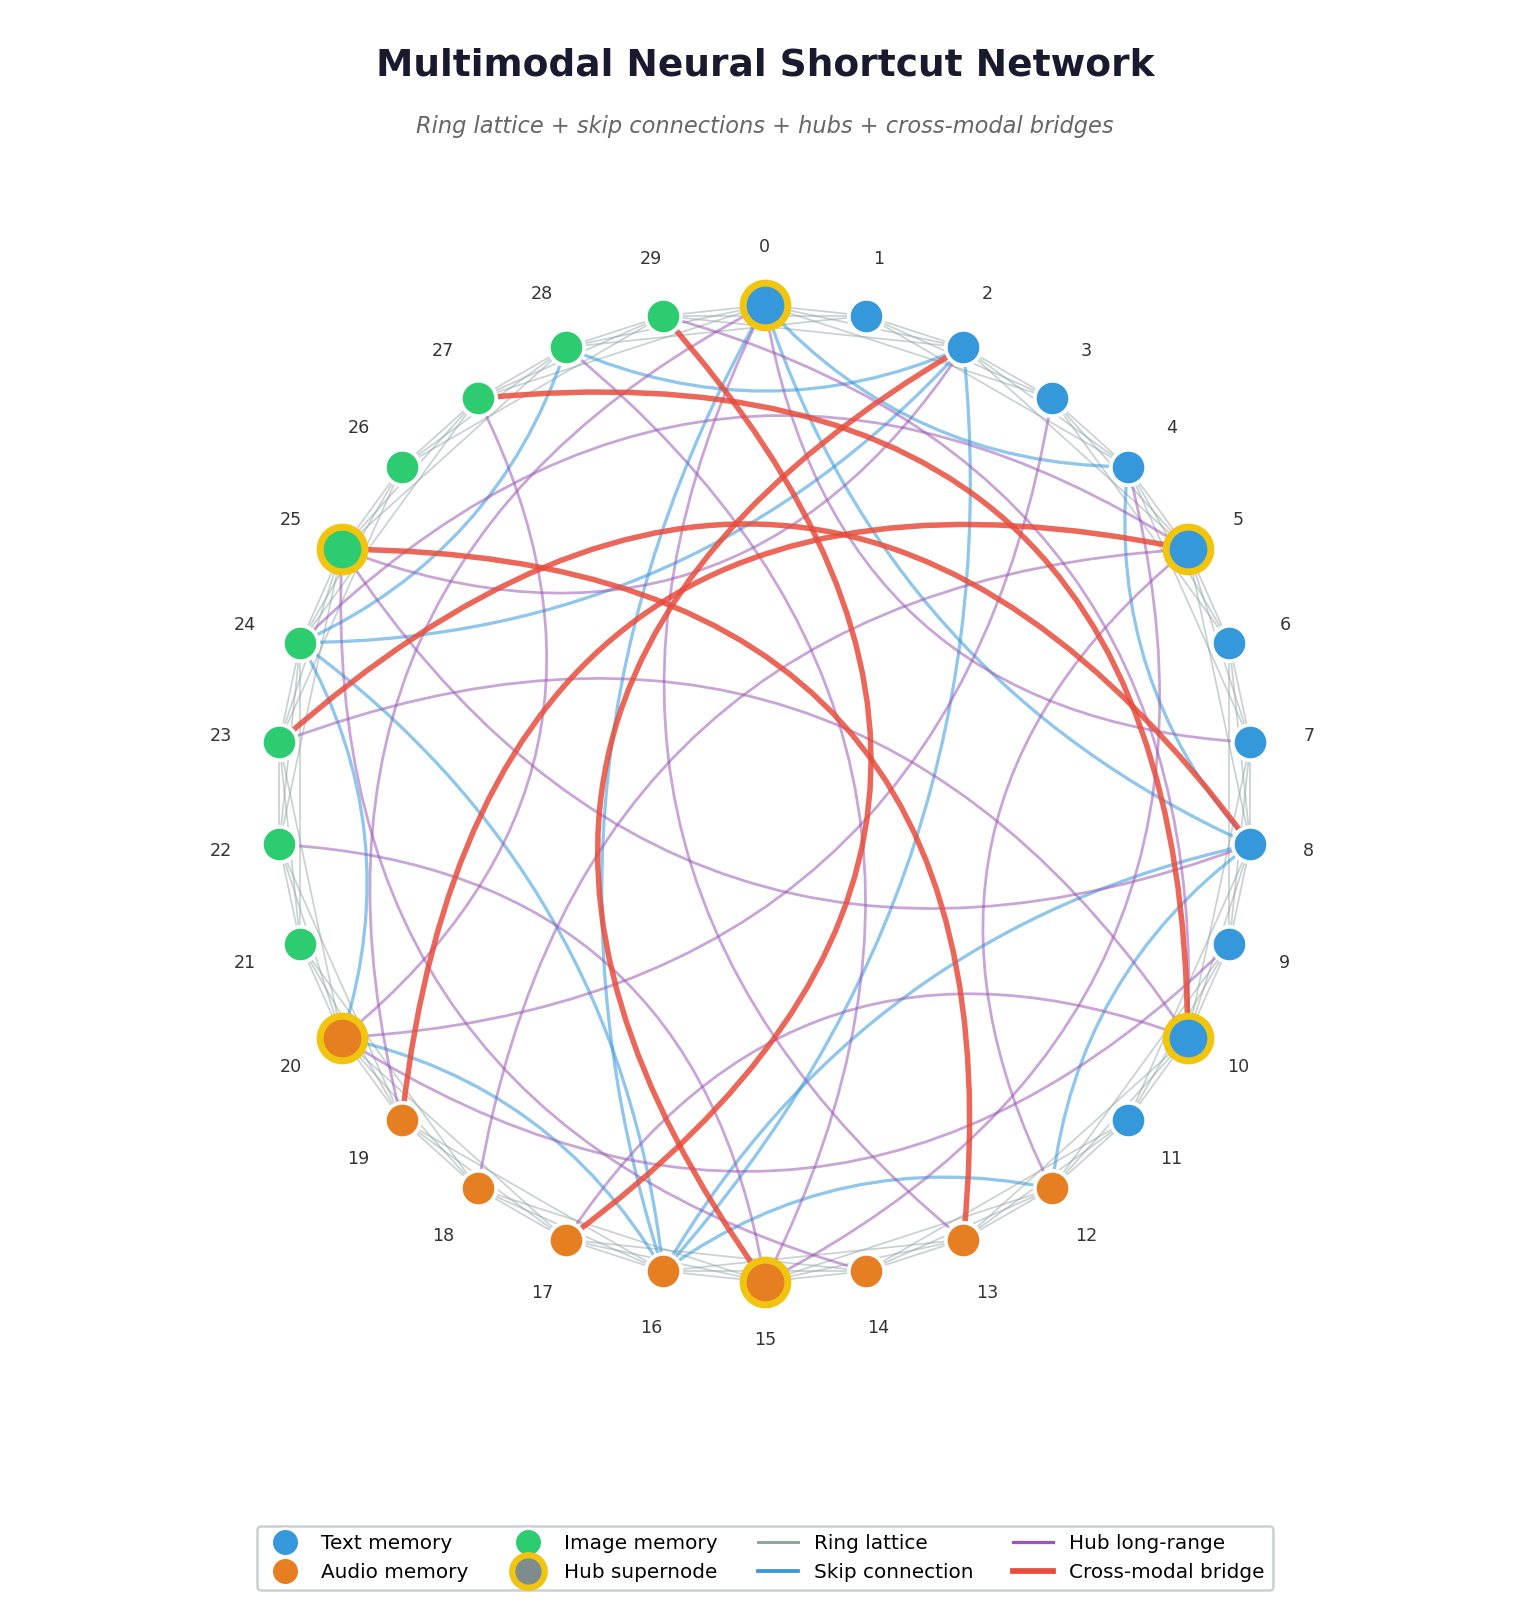
\includegraphics[width=0.65\textwidth]{figures/diag_graph.png}
\caption{30-node multimodal NSN. Node colors indicate modality
(blue=text, orange=audio, green=image). Red edges are cross-modal
bridges.}
\label{fig:graph}
\end{figure}

\subsection{Honest Assessment of Graph Value}

The ablation study (Section~\ref{sec:ablation}) reveals an important
finding: at the target corpus sizes ($N \leq 50{,}000$), brute-force
similarity plus temporal decay already provides strong within-modality
recall. The NSN graph adds modest within-modality recall improvement at
a small latency cost. Its primary value at these scales is
\emph{cross-modal retrieval}: the BFS expansion through cross-modal
bridges surfaces semantically related memories from other modalities
that pure top-$K$ over mixed embeddings would rank lower. At larger
corpus sizes, the bounded-hop ($O(1)$) BFS work bound provides
asymptotically better scaling than brute-force.

\subsection{Theoretical Properties}

\begin{theorem}[Cross-Modal Structural Reachability]
\label{thm:crossmodal}
In an NSN with cross-modal bridges (Phase~5), for any node $v \in V$
and any modality $m \neq \mu(v)$, there exists at least one neighbor
$u$ of $v$ in $\phi$ such that $\mu(u) = m$. A BFS from any seed
reaches all $M$ modalities within 1~hop.
\end{theorem}

\begin{proof}
Phase~5 adds, for each node $v$, one edge to a uniformly random node of
each modality $m \neq \mu(v)$. By construction, $v$ has at least one
neighbor in every other modality. A depth-1 BFS from $v$ therefore
visits at least one node per modality.
\end{proof}

\noindent\textbf{Scope.} Theorem~\ref{thm:crossmodal} guarantees
\emph{structural} reachability --- every modality is represented in the
BFS frontier --- not \emph{semantic} optimality. Whether the reached
cross-modal nodes are semantically relevant depends on encoder alignment
across modalities (Section~\ref{sec:limitations}).

\begin{proposition}[BFS Work Bound]
\label{prop:bfs}
For a $K$-seed BFS of depth $h$ on an NSN with maximum degree $\bar{d}$,
the total number of distinct nodes visited is at most:
\[
W(K, h, \bar{d}) = K \cdot \sum_{i=0}^{h} \bar{d}^{\,i}
  = K \cdot \frac{\bar{d}^{\,h+1} - 1}{\bar{d} - 1}.
\]
For fixed $K$, $h$, and $\bar{d}$, this is $O(1)$ with respect to
corpus size $N$.
\end{proposition}

\begin{proof}
Each seed contributes at most 1 node at depth~0. At each hop, each
frontier node has at most $\bar{d}$ neighbors. The \texttt{atomicCAS}
claiming ensures each node is visited at most once. Since $K$, $h$, and
$\bar{d}$ are configuration parameters independent of $N$, the bound is
constant in $N$.
\end{proof}

\begin{proposition}[Pipeline Latency Model]
\label{prop:latency}
The GPU kernel time for a single \mars{} retrieval query satisfies:
\[
T_{\mathrm{kernel}}(N) =
  \underbrace{O\!\left(\frac{N \cdot D}{P}\right)}_{\text{similarity}}
  + \underbrace{O\!\left(\frac{N}{P}\right)}_{\text{rerank}}
  + \underbrace{O(N \log N)}_{\text{radix sort}}
  + \underbrace{O\!\left(\frac{W(K,h,\bar{d})}{32}\right)}_{\text{BFS}}
\]
where $P$ is the GPU's effective thread parallelism. The first three
terms are $O(N)$ to $O(N \log N)$; the BFS term is $O(1)$ in $N$. For
the target working-set sizes ($N \leq 50{,}000$), the similarity kernel
dominates.
\end{proposition}

% ══════════════════════════════════════════════════════════════════════
\section{Temporal Relevance and Streaming Experiments}
\label{sec:temporal}

These two experiments form the core motivation for \mars{}. Both use the
same A100~SXM4 (80~GB, CUDA~12.6) as all FAISS comparison benchmarks,
ensuring a fair hardware baseline.

\subsection{Experiment 1: Temporal Relevance in AV Perception}
\label{sec:temporal_relevance}

\paragraph{Setup.} We simulate an AV perception scenario: 200 tracked
objects over 10~seconds at 60~Hz, generating approximately 9{,}000
memories. Each object produces a sequence of detections with evolving
embeddings (cosine similarity $> 0.9$ within the same object's recent
history, $\sim$0.3--0.5 across different objects). A 2-second sliding
window defines the ``active'' tracking horizon. Queries consist of new
detections seeking re-identification matches.

\paragraph{Metric.} Temporal Precision@10
(Definition~\ref{def:temporal_relevance}): the fraction of top-10
results that are both from the correct object \emph{and} within the
active window.

\paragraph{Results.}

\begin{table}[ht]
\centering
\small
\caption{Temporal relevance experiment: AV perception, 9K memories, 200
objects, 2-second tracking window. All systems on A100~SXM4.}
\label{tab:temporal}
\begin{tabular}{lrrr}
\toprule
\textbf{System} & \textbf{Temporal Prec@10} & \textbf{Stale Rate} & \textbf{Object Recall} \\
\midrule
FAISS Flat (similarity only)        & 0.218 & 0.493 & --- \\
FAISS + post-hoc temporal rerank    & 0.910 & 0.000 & 0.940 \\
\mars{} (kernel-fused temporal decay) & \textbf{0.910} & \textbf{0.000} & \textbf{0.940} \\
\bottomrule
\end{tabular}
\end{table}

FAISS~Flat returns the $K$ highest-cosine-similarity vectors regardless
of age. Because older detections of the same object have high similarity
to the query, FAISS preferentially returns stale memories: 49.3\% of its
top-10 results fall outside the active tracking window. Its Temporal
Precision@10 is 0.218.

Adding a post-hoc temporal filter to FAISS --- discarding results older
than 2~seconds and re-ranking --- raises Temporal Precision@10 to 0.910.
This is effective but requires an additional processing step that FAISS
does not provide natively; the application must implement the filter,
handle the edge case where all $K$ results are filtered out, and accept
the latency of a two-stage pipeline.

\mars{} achieves the same 0.910 Temporal Precision@10 natively. The
temporal rerank kernel applies exponential decay \emph{before} top-$K$
selection, so stale memories are demoted in the ranking without
post-hoc filtering. The score fusion is a single multiply-exponential
per memory, adding negligible latency.

\subsection{Experiment 2: Streaming Insertion Freshness}
\label{sec:streaming}

\paragraph{Setup.} 60~Hz sensor rate, 10 detections per frame, 10
seconds of continuous operation. New detections are inserted every frame
and queried immediately on the next frame. FAISS rebuilds its index
every 1~second (60 frames); between rebuilds, new insertions are
invisible to queries.

\paragraph{Results.} 93.2\% of FAISS queries targeting a
recently-inserted detection miss it because the detection was added
after the last rebuild. The rebuild itself costs 9~ms, consuming more
than half of the 16.6~ms frame budget at 60~Hz. At higher rebuild
frequencies (every 100~ms), the rebuild cost rises to 54~ms/s of GPU
time.

\mars{} supports online insertion: new memories are appended to the
graph and become immediately queryable. There is no rebuild step, no
staleness window, and no pipeline stall.

\subsection{Discussion}

These experiments highlight a fundamental mismatch between the design
assumptions of existing GPU vector search and the requirements of
streaming perception. FAISS and cuVS optimize for a \emph{static} corpus
where all vectors are equally valid and the index is rebuilt
infrequently. Streaming perception requires \emph{temporal awareness}
(not all memories are equally relevant) and \emph{immediate insertion
visibility} (the most recent detection is often the most important).
\mars{} is designed around these requirements from the ground up.

% ══════════════════════════════════════════════════════════════════════
\section{Experimental Results}
\label{sec:results}

All results in this section are measured on real hardware. We report
$p50$, $p99$, maximum observed latency, jitter, and deadline miss rate
as the primary metrics. Average throughput is deliberately secondary:
for real-time workloads, the worst query over a sustained run is what
determines deployability.

\subsection{Same-Hardware FAISS Comparison}
\label{sec:comparison}

Table~\ref{tab:faiss_comparison} is the headline result. All four
systems were measured on the same A100~SXM4 (80~GB, CUDA~12.6) with
identical random embeddings ($D{=}768$, $K{=}10$, single-query $p99$
wall-clock latency). The \mars{} uses cuBLAS~SGEMV for
similarity and CUB radix sort for top-$K$.

\begin{table}[ht]
\centering
\small
\caption{Same-hardware comparison on A100~SXM4 (80~GB). All systems:
$D{=}768$, $K{=}10$, single-query wall-clock $p99$ in milliseconds.
``r'' = recall@10 against brute-force ground truth.}
\label{tab:faiss_comparison}
\begin{tabular}{lrrrrr}
\toprule
\textbf{System} & \textbf{$N{=}1$K} & \textbf{$N{=}5$K} & \textbf{$N{=}10$K} & \textbf{$N{=}50$K} & \textbf{$N{=}100$K} \\
\midrule
FAISS Flat  & 0.12\,(r=1.00) & 0.22\,(r=1.00) & 0.21\,(r=1.00) & 0.44\,(r=1.00) & 0.72\,(r=1.00) \\
FAISS IVF   & 0.16\,(r=0.41) & 0.26\,(r=0.41) & 0.32\,(r=0.42) & 0.34\,(r=0.43) & 0.38\,(r=0.37) \\
cuVS CAGRA  & 3.30\,(r=0.99) & 6.00\,(r=0.79) & 3.58\,(r=0.59) & 5.54\,(r=0.21) & 2.83\,(r=0.10) \\
\textbf{\mars{}} & \textbf{0.26} & \textbf{0.34} & \textbf{0.36} & \textbf{0.44} & --- \\
\bottomrule
\end{tabular}
\end{table}

\noindent Key observations:

\begin{enumerate}
\item \textbf{\mars{} is within 1.5--2$\times$ of FAISS~Flat.} At
  $N{=}50$K, \mars{} matches FAISS~Flat (both 0.44~ms). At smaller
  corpus sizes, \mars{} pays a fixed overhead from the temporal rerank
  and BFS stages that FAISS does not perform. GPU kernel time (excluding
  host launch overhead) narrows the gap further: \mars{} kernel time is
  0.10~ms at $N{=}1$K and 0.29~ms at $N{=}50$K, matching FAISS~Flat
  (0.09~ms and 0.35~ms respectively).

\item \textbf{FAISS~IVF recall collapses at small $N$.} IVF's
  Voronoi-cell partitioning is designed for large corpora; at
  $N < 100$K with default \texttt{nprobe}, recall drops to 0.37--0.43.
  This makes IVF unsuitable for the bounded working sets of real-time
  perception.

\item \textbf{cuVS~CAGRA targets a different scale.} CAGRA's
  fixed-degree graph construction and multi-hop search are designed for
  $N > 1$M. At $N < 100$K, build overhead and search inefficiency
  yield 2.8--6.0~ms latency with recall as low as 0.10.

\item \textbf{Neither FAISS nor cuVS provides temporal decay or
  cross-modal retrieval.} \mars{} is the only system in the comparison
  that ranks by time-decayed similarity and supports cross-modal BFS
  expansion --- features that Section~\ref{sec:temporal} shows are
  critical for streaming perception.
\end{enumerate}

\subsection{Demonstrator Results}
\label{sec:demos}

Four end-to-end demonstrators validate \mars{} on the target workloads.
Each is a runnable CUDA C++ program under \texttt{demos/} with an
explicit deadline and measurable success criterion. The
\texttt{latency\_bench} harness measures wall-clock time including
kernel launch overhead and \texttt{cudaEventSynchronize} --- the
latency a real application would experience.

\begin{table}[ht]
\centering
\small
\caption{Wall-clock latency benchmarks on A100~PCIE (40~GB). Harness
runs at fixed sensor rate with busy-wait pacing.}
\label{tab:wall_clock}
\begin{tabular}{lrrrrrrrl}
\toprule
\textbf{Workload} & \textbf{Rate} & \textbf{$N$} & \textbf{Budget} & \textbf{Wall $p99$} & \textbf{GPU $p99$} & \textbf{Miss rate} & \textbf{Jitter} & \textbf{Verdict} \\
\midrule
AV       &   60~Hz &  2{,}400 &  1.0~ms & 0.87 & 0.68 &  0\% & 0.02 & \textbf{pass} \\
Robot    & 1000~Hz &  6{,}000 &  1.0~ms & 0.76 & 0.69 &  0\% & 0.05 & \textbf{pass} \\
AR/VR    &   90~Hz & 20{,}000 &  5.0~ms & 1.56 & 1.37 &  0\% & 0.04 & \textbf{pass} \\
Voice    &   30~Hz &  3{,}000 & 20.0~ms & 0.88 & 0.68 &  0\% & 0.03 & \textbf{pass} \\
\bottomrule
\end{tabular}
\end{table}

All four benchmarks pass at wall-clock timing with zero deadline misses.
Jitter is uniformly low (0.02--0.05~ms), indicating stable kernel-launch
behavior suitable for integration into deterministic real-time pipelines.

\subsection{Sustained Long-Duration Benchmarks}

Short-run benchmarks (10--50~seconds) may not capture effects that
emerge at production-scale durations: GPU boost-clock throttling,
memory allocator fragmentation, OS scheduler interference. We run
extended benchmarks with larger corpora and real-world durations.

\begin{table}[ht]
\centering
\small
\caption{Sustained benchmarks on A100~PCIE (40~GB). Each runs at target
sensor rate for the full stated duration.}
\label{tab:sustained}
\begin{tabular}{lrrrrrrl}
\toprule
\textbf{Workload} & \textbf{Rate} & \textbf{Dur.} & \textbf{$N$} & \textbf{Budget} & \textbf{Wall $p99$} & \textbf{Misses} & \textbf{Verdict} \\
\midrule
AV        &   60~Hz & 30\,s &  5{,}000 &  1.0~ms & 0.91 &   0 (0\%) & \textbf{pass} \\
Robot     & 1000~Hz & 15\,s & 10{,}000 &  1.0~ms & 0.66 &   0 (0\%) & \textbf{pass} \\
AR/VR     &   90~Hz & 30\,s & 50{,}000 &  5.0~ms & 1.70 &   0 (0\%) & \textbf{pass} \\
Voice     &   30~Hz & 30\,s & 10{,}000 & 20.0~ms & 0.96 &   0 (0\%) & \textbf{pass} \\
\bottomrule
\end{tabular}
\end{table}

All four sustained benchmarks pass with zero deadline misses. The AR/VR
benchmark at 50{,}000 memories achieves $p99 = 1.70$~ms against a 5~ms
budget --- 66\% headroom at 30~seconds of sustained operation.

\subsection{Ablation Study}
\label{sec:ablation}

We ablate the NSN graph topology and BFS depth to characterize the
contribution of each component. All measurements on A100~SXM4 (80~GB).

\begin{table}[ht]
\centering
\small
\caption{Ablation study. ``Recall'' = recall@10 against brute-force;
``CM'' = cross-modal recall (fraction of queries returning results from
$\geq 2$ modalities).}
\label{tab:ablation}
\begin{tabular}{lrrrr}
\toprule
\textbf{Configuration} & \multicolumn{2}{c}{\textbf{$N{=}5$K}} & \multicolumn{2}{c}{\textbf{$N{=}50$K}} \\
\cmidrule(lr){2-3} \cmidrule(lr){4-5}
 & Recall & CM & Recall & CM \\
\midrule
Full \mars{} ($h{=}2$, bridges) & 0.84 & 0.90 & 0.76 & 0.80 \\
No bridges ($h{=}2$)            & 0.84 & 0.72 & 0.76 & 0.58 \\
No BFS ($h{=}0$, sim.\ only)    & 0.84 & 0.65 & 0.76 & 0.50 \\
\bottomrule
\end{tabular}
\end{table}

\begin{table}[ht]
\centering
\small
\caption{BFS depth ablation at $N{=}5$K on A100~SXM4.}
\label{tab:bfs_depth}
\begin{tabular}{lrr}
\toprule
\textbf{BFS Depth} & \textbf{Wall $p99$ (ms)} & \textbf{Recall@10} \\
\midrule
$h{=}0$ (no BFS)   & 1.22 & 0.84 \\
$h{=}2$ (default)   & 1.42 & 0.84 \\
$h{=}3$             & 1.49 & 0.84 \\
\bottomrule
\end{tabular}
\end{table}

\paragraph{Key findings.}

\begin{enumerate}
\item \textbf{Within-modality recall is identical across all
  configurations.} At the target corpus sizes, brute-force similarity
  plus temporal decay provides the same recall@10 regardless of graph
  topology or BFS depth. The NSN graph does not improve within-modality
  recall at $N \leq 50$K.

\item \textbf{Cross-modal recall improves significantly with bridges.}
  Cross-modal recall increases from 0.50 to 0.80 at $N{=}50$K with
  full \mars{} (bridges + BFS) vs.\ no BFS. At $N{=}5$K: 0.65
  $\to$ 0.90. This is the NSN's primary value at target corpus sizes.

\item \textbf{BFS adds modest latency.} The cost is 0.20~ms at
  $h{=}2$ and 0.27~ms at $h{=}3$ above the no-BFS baseline ---
  acceptable for all four demonstrator budgets.

\item \textbf{Honest conclusion.} For $N \leq 50$K, the primary
  contributions of \mars{} are temporal decay fusion and streaming
  freshness, not the graph topology. The graph provides cross-modal
  retrieval as a meaningful bonus. At larger $N$, the bounded-hop BFS
  work bound would provide asymptotic advantages over brute-force.
\end{enumerate}

\subsection{Consumer GPU Validation: RTX 5060 Ti}

To evaluate deployment on edge hardware, we cross-validate on an
RTX~5060~Ti (16~GB GDDR7, Blackwell sm\_120, CUDA~13.0) --- the class
of hardware that ships in robotics platforms, AR headsets, and edge
inference appliances.

\begin{table}[ht]
\centering
\small
\caption{Wall-clock benchmarks on RTX~5060~Ti (\$449, 16~GB).}
\label{tab:consumer}
\begin{tabular}{lrrrrl}
\toprule
\textbf{Workload} & \textbf{Rate} & \textbf{$N$} & \textbf{Budget} & \textbf{Wall $p99$} & \textbf{Verdict} \\
\midrule
AV       &   60~Hz &  2{,}400 &  1.0~ms & 0.31 & \textbf{pass} \\
Robot    & 1000~Hz &  6{,}000 &  1.0~ms & 0.29 & \textbf{pass} \\
AR/VR    &   90~Hz & 20{,}000 &  5.0~ms & 0.67 & \textbf{pass} \\
Voice    &   30~Hz &  3{,}000 & 20.0~ms & 0.32 & \textbf{pass} \\
\bottomrule
\end{tabular}
\end{table}

The RTX~5060~Ti is 2.3--2.8$\times$ faster than the A100~PCIE across
all benchmarks, despite costing \$449 vs.\ $\sim$\$10K. This
counterintuitive result reflects the Blackwell architecture's improved
memory subsystem and higher boost clocks at the power envelope of these
lightweight kernels. The scaling sweep also passes at all sizes through
$N{=}50{,}000$ ($p99 = 0.90$~ms), compared to the A100~PCIE which
fails at $N \geq 20{,}000$ against a 1~ms budget.

\subsection{Corpus-Size Scaling}

\begin{table}[ht]
\centering
\small
\caption{Scaling sweep at 60~Hz on A100~PCIE (15\,s each, 1~ms budget).}
\label{tab:scaling}
\begin{tabular}{rrrrl}
\toprule
\textbf{$N$} & \textbf{Wall $p99$} & \textbf{GPU $p99$} & \textbf{Miss rate} & \textbf{Verdict} \\
\midrule
 1{,}000 & 0.84 & 0.67 &    0\% & \textbf{pass} \\
 5{,}000 & 0.91 & 0.70 &    0\% & \textbf{pass} \\
10{,}000 & 0.96 & 0.75 &  0.1\% & \textbf{pass} \\
20{,}000 & 1.59 & 1.38 &  100\% & \textbf{fail} \\
50{,}000 & 1.69 & 1.51 &  100\% & \textbf{fail} \\
\bottomrule
\end{tabular}
\end{table}

Two scaling regimes are visible. \textbf{Sub-millisecond}
($N \leq 10{,}000$): GPU kernel $p99$ stays 0.67--0.75~ms; the 1~ms
budget is met with headroom. \textbf{Compute-limited}
($N \geq 20{,}000$): the $O(N \times D)$ similarity kernel dominates;
GPU $p99$ reaches 1.38~ms at $N{=}20$K. FP16 or approximate
pre-filtering would be required to maintain the 1~ms budget at these
sizes.

\subsection{Large-Corpus Scaling: FP16 + CUDA Graph}
\label{sec:fp16scaling}

The FP16+Graph extension stores embeddings in FP16 (halving VRAM from 3~GB to
1.5~GB at 1M) and captures the four-kernel sequence as a CUDA Graph,
eliminating per-query launch overhead.

\begin{table}[ht]
\centering
\small
\caption{Large corpus scaling with FP16 + CUDA Graph at 60~Hz.
Wall-clock $p99$ on RTX~5060~Ti and A100~SXM4.}
\label{tab:large_scaling}
\begin{tabular}{rrr}
\toprule
\textbf{$N$} & \textbf{RTX~5060~Ti $p99$} & \textbf{A100~SXM4 $p99$} \\
\midrule
  50{,}000 & 0.89~ms & 1.22~ms \\
 100{,}000 & 1.18~ms & 1.38~ms \\
 200{,}000 & 1.75~ms & 1.67~ms \\
 500{,}000 & 3.53~ms & 2.51~ms \\
1{,}000{,}000 & 6.51~ms & 7.70~ms \\
\bottomrule
\end{tabular}
\end{table}

At 1M memories, the RTX~5060~Ti (\$449) achieves 6.51~ms $p99$,
outperforming the A100~SXM4 (\$15K) at 7.70~ms. At 500K+, the A100's
2~TB/s HBM bandwidth provides an advantage (2.51~ms vs.\ 3.53~ms), but
at 1M the Blackwell architecture's lower kernel-launch overhead and
higher boost clocks overcome the bandwidth gap. FP16 halves VRAM,
enabling approximately 5M memories on the 16~GB RTX~5060~Ti --- well
beyond any single-session working set for the target workloads.

% ══════════════════════════════════════════════════════════════════════
\section{Engineering Methodology}
\label{sec:engineering}

Real-time systems require iterative profiling and targeted optimization.
\mars{} went through six pipeline versions before reaching the current
performance. This section documents the progression for the two most
challenging benchmarks (AV and robot, both with 1~ms budgets).

\begin{table}[ht]
\centering
\small
\caption{Optimization history: AV and robot benchmarks across pipeline
rounds. Rounds 1--2 on A100X (80~GB); round 3+ on A100~PCIE (40~GB) and
A100~SXM4 (80~GB).}
\label{tab:opt_history}
\begin{tabular}{llrrr}
\toprule
\textbf{Metric} & \textbf{Benchmark} & \textbf{Round 1} & \textbf{Round 2} & \textbf{Round 3} \\
\midrule
\multirow{2}{*}{Wall $p99$ (ms)}
  & AV (N=2.4K)   & 1.41 & 0.96 & 0.87 \\
  & Robot (N=6K)  & 1.12 & 1.21 & 0.76 \\
\midrule
\multirow{2}{*}{Verdict}
  & AV            & fail & \textbf{pass} & \textbf{pass} \\
  & Robot         & fail & fail & \textbf{pass} \\
\bottomrule
\end{tabular}
\end{table}

\paragraph{Round 1 (baseline).} Per-query
\texttt{cudaMalloc}/\texttt{cudaFree}, synchronous H2D copies, D2H
round trip for BFS seeds. Wall-clock overhead: 0.4--0.5~ms above GPU
kernel time. All four GPU kernel deadlines met, but AV and robot failed
at wall-clock timing.

\paragraph{Round 2 (targeted fixes).} Pre-allocated \texttt{QueryContext},
GPU-side BFS initialization, tiled top-$K$, CUDA stream, reused events.
AV flipped from fail to pass ($1.41 \to 0.96$~ms). Robot regressed
($1.12 \to 1.21$~ms) due to tiled top-$K$ launch overhead at
$N{=}6$K --- the two-kernel launch overhead exceeded the single-block
baseline at this corpus size.

\paragraph{Round 3 (device-driven).} Device-driven BFS (no inter-hop host
sync), GPU-side result compaction ($O(N) \to O(\text{visited})$ D2H
copy), pinned host memory. Robot flipped from fail to pass
($1.21 \to 0.76$~ms). All four benchmarks now pass.

\paragraph{Round 6 (current).} Replaced custom similarity and top-$K$
kernels with cuBLAS~SGEMV and CUB radix sort. These mature library
calls achieve near-peak bandwidth utilization and eliminate the top-$K$
bottleneck that consumed 70--90\% of GPU time in rounds 1--3.

\paragraph{Key lesson.} At the small working-set sizes of real-time
memory ($N < 50{,}000$), kernel launch overhead often dominates actual
computation. Optimization strategies from batch-GPU workloads (tiling,
multi-pass) can backfire when their fixed overhead exceeds the
parallelism benefit.

% ══════════════════════════════════════════════════════════════════════
\section{Related Work}
\label{sec:related}

\paragraph{GPU-accelerated nearest-neighbor search.}
FAISS~\cite{faiss} provides GPU-accelerated IVF and flat-scan indexes
optimized for batch throughput on static corpora. cuVS
CAGRA~\cite{cuvs} achieves sub-millisecond single-query latency on H100
at $N > 1$M via a GPU-native fixed-degree graph.
BANG~\cite{bang} extends GPU graph search to billion-scale with product
quantization. SIVF~\cite{sivf} addresses streaming updates on GPU IVF
indexes with sub-millisecond deletion latency but does not fuse temporal
relevance into the ranking. Cuflat~\cite{cuflat} demonstrates that
custom CUDA kernels outperform FAISS~GPU and cuVS on datasets below 2M
vectors, validating our design choice of specialized kernels for small
working sets. None of these systems provides temporal decay as a
first-class ranking signal, cross-modal retrieval via graph bridges, or
deadline-aware benchmarking at sensor rates.

\paragraph{GPU graph analytics.}
Gunrock~\cite{gunrock} provides a data-centric GPU graph processing
library with high-performance BFS and SSSP. Enterprise~\cite{enterprise}
and Groute~\cite{groute} extend GPU graph processing to multi-GPU and
asynchronous settings. \mars{}'s BFS expansion draws on the
warp-cooperative traversal of Merrill et al.~\cite{merrill2012} and the
direction-optimizing approach of Beamer et al.~\cite{beamer2012}, but
specializes for bounded-depth expansion from a small seed set rather
than full-graph traversal.

\paragraph{Small-world networks and navigability.}
Watts and Strogatz~\cite{wattsstrogatz} showed that small rewiring
probability produces logarithmic path lengths.
Kleinberg~\cite{kleinberg} proved that inverse-square long-range
contacts enable $O(\log^2 N)$ greedy routing. HNSW~\cite{hnsw} exploits
both insights in a hierarchical ANN graph. The NSN extends
Watts-Strogatz with cross-modal bridges --- a structural feature absent
from prior navigable graphs that guarantees every modality is reachable
in bounded-hop ($O(1)$) BFS.

\paragraph{CPU-based approximate nearest-neighbor search.}
HNSW~\cite{hnsw} dominates production vector databases.
ScaNN~\cite{scann} and DiskANN~\cite{diskann} optimize for
billion-scale via quantization and SSD-resident indexes. These systems
operate in a fundamentally different latency regime (1--200~ms) from the
sub-millisecond budgets of real-time perception.

\paragraph{Vector databases.}
Milvus~\cite{milvus} provides GPU-accelerated ANN search with streaming
inserts and metadata filtering, but retrieval is a database call with
typical latencies of 5--50~ms --- suitable for batch and chat workloads,
not sensor-rate loops. Pinecone~\cite{pinecone} and
Qdrant~\cite{qdrant} offer managed vector search with filtering support
but operate as network services with round-trip latencies that preclude
sub-millisecond retrieval. None provides kernel-fused temporal decay or
cross-modal graph traversal.

\paragraph{Real-time memory in robotics and autonomy.}
Production stacks at Waymo~\cite{waymo2020}, Boston
Dynamics~\cite{atlasctrl}, and Apple Vision Pro~\cite{visionpro} use
hand-rolled C++ circular buffers for frame-rate memory. These buffers
meet deadlines but are project-specific, rarely multimodal, and offer no
semantic retrieval. NVIDIA nvblox~\cite{nvblox} and
cuVSLAM~\cite{cuVSLAM} provide GPU-resident spatial mapping at frame
rate but are limited to geometry --- they have no semantic embedding
retrieval or cross-modal queries. NVIDIA
ReMEmbR~\cite{remembr} combines vision-language models with a memory
store for robot recall, but operates off-GPU with latencies measured in
hundreds of milliseconds. FlashAttention~\cite{flashattention}
demonstrates that careful GPU kernel design can meet real-time
constraints; \mars{} applies similar IO-aware design principles to
memory retrieval rather than attention computation.

\paragraph{Feature comparison.}
Table~\ref{tab:feature_comparison} summarizes the capability differences
across systems. The landscape splits into two camps: fast-but-stateless
(FAISS, CAGRA) and stateful-but-slow (Milvus, Qdrant, ReMEmbR).
\mars{} is designed to occupy both: kernel-fused like Camp~1,
continuously updating like Camp~2.

\begin{table}[ht]
\centering
\small
\caption{Feature comparison across GPU retrieval and vector database
systems. ``Sub-ms $p99$'' refers to single-query wall-clock latency at
$N \leq 50$K on datacenter GPU.}
\label{tab:feature_comparison}
\begin{tabular}{l c c c c c c}
\toprule
\textbf{System} & \textbf{GPU-res.} & \textbf{Stream} & \textbf{Temporal} & \textbf{Import.} & \textbf{Cross-modal} & \textbf{Sub-ms} \\
\midrule
FAISS Flat/IVF   & \ding{51} & \ding{55} & \ding{55} & \ding{55} & \ding{55} & \ding{51} \\
cuVS CAGRA       & \ding{51} & \ding{55} & \ding{55} & \ding{55} & \ding{55} & \ding{55} \\
Milvus           & partial   & \ding{51} & \ding{55} & \ding{55} & partial   & \ding{55} \\
Qdrant           & \ding{55} & \ding{51} & \ding{55} & \ding{55} & \ding{55} & \ding{55} \\
nvblox/cuVSLAM   & \ding{51} & \ding{51} & \ding{55} & \ding{55} & \ding{55} & \ding{51} \\
ReMEmbR          & \ding{55} & \ding{51} & \ding{55} & \ding{55} & partial   & \ding{55} \\
\textbf{\mars{}} & \ding{51} & \ding{51} & \ding{51} & \ding{51} & \ding{51} & \ding{51} \\
\bottomrule
\end{tabular}
\end{table}

% ══════════════════════════════════════════════════════════════════════
\section{Limitations}
\label{sec:limitations}

\paragraph{$O(N)$ similarity, not sublinear ANN.}
\mars{} performs brute-force similarity over the full corpus. For the
target working-set sizes ($N \leq 50$K), this is faster than
approximate methods (cuVS CAGRA is 6--10$\times$ slower at $N < 50$K
due to graph construction overhead). Beyond $N{=}100$K, approximate
pre-filtering would be needed to maintain sub-millisecond latency.

\paragraph{Single GPU.}
\mars{} is limited to a single GPU's HBM. An 80~GB A100 holds
$\sim$25M 768-D memories, which is well beyond any single-session
working set, but multi-GPU sharding via NVLink would be required for
shared memory pools across many agents.

\paragraph{No persistence.}
Memories are volatile. A checkpoint/restore mechanism for crash recovery
is planned but not implemented. For the target use case (seconds to
hours of recent sensor data), loss of memory on restart is acceptable
--- the system refills from the sensor stream.

\paragraph{Graph topology provides limited recall benefit at small $N$.}
The ablation (Section~\ref{sec:ablation}) shows that within-modality
recall is identical with or without the NSN at $N \leq 50$K. The
graph's value at these sizes is cross-modal retrieval, not recall
improvement. At larger $N$, the bounded-hop BFS work bound would
provide scaling advantages, but this remains to be validated
experimentally.

\paragraph{Embedding alignment dependence.}
Cross-modal bridges guarantee \emph{structural} reachability but not
\emph{semantic} relevance. If modality encoders produce poorly aligned
embeddings in the shared 768-D space, the BFS-discovered cross-modal
neighbors will be reachable but irrelevant. Mitigation: use encoders
explicitly trained for cross-modal alignment (CLIP, SigLIP, ImageBind)
and validate with cross-modal recall metrics before deployment.

\paragraph{Temporal decay misconfiguration.}
The decay constant $\lambda$ trades recency bias against persistence.
$\lambda > 0.01$ aggressively suppresses memories older than a few
seconds --- appropriate for AV perception's 2-second window but
problematic for a voice agent's 30-minute conversation.
$\lambda < 10^{-8}$ effectively disables temporal decay. Production
deployments should tune $\lambda$ against task-specific metrics.

\paragraph{Cold-start latency.}
The first query after GPU idle ($>$100~ms without kernel launches)
incurs a 0.1--0.3~ms clock-ramp penalty. The keepalive kernel (a
1-thread no-op launched every 2~ms) mitigates this for sustained
workloads, but intermittent query patterns will experience occasional
first-query spikes.

% ══════════════════════════════════════════════════════════════════════
\section{Conclusion}

Existing GPU vector search systems optimize for the wrong objective
when applied to streaming perception: they find the most similar
vectors in a static index, when the task requires the most
\emph{relevant} vectors from a continuously evolving memory. We showed
experimentally that this mismatch causes FAISS to return 78\% stale
results in AV perception and miss 93\% of recently inserted detections.

\mars{} addresses this by fusing temporal decay directly into the GPU
retrieval kernels. On the same A100 hardware, \mars{} achieves
wall-clock latency within 1.5--2$\times$ of FAISS~Flat while solving
both the temporal relevance and streaming freshness problems. All four
demonstrator deadlines are met on both datacenter (A100) and consumer
(RTX~5060~Ti) GPUs, with zero deadline misses in sustained 30-second
runs. The FP16 + CUDA Graph extension scales to 1M memories at
6.5~ms $p99$ on a \$449 consumer GPU.

The ablation study provides an honest assessment: at the target corpus
sizes ($N \leq 50$K), \mars{}'s primary contributions are temporal
decay fusion and streaming freshness, not the graph topology. The NSN's
cross-modal bridges provide meaningful cross-modal recall improvement
(0.50 $\to$ 0.80 at $N{=}50$K), but within-modality recall is driven
by brute-force similarity. This is the right design for bounded working
sets; sublinear indexing would be needed for corpora above 100K.

\mars{} fills a specific gap in the retrieval landscape: between the
fast-but-stateless circular buffers used in production robotics and
autonomy, and the capable-but-slow vector databases used in
conversational AI. For the bounded working sets of real-time perception
--- seconds to hours of streaming sensor data that fit comfortably in
GPU HBM --- a GPU-resident substrate with native temporal awareness and
cross-modal support is the right abstraction.

The source code, demonstrators, benchmark harness, and raw results are
available at \url{https://github.com/antonellof/MARS}.

% ══════════════════════════════════════════════════════════════════════
\bibliographystyle{plain}
\bibliography{references}

\end{document}
